\documentclass[border=8pt]{standalone}
\usepackage[T1]{fontenc}
\usepackage{amsmath,amssymb}
\usepackage{xcolor}
\usepackage{tikz}
\usetikzlibrary{shapes,arrows,positioning,fit,backgrounds,calc}
\begin{document}
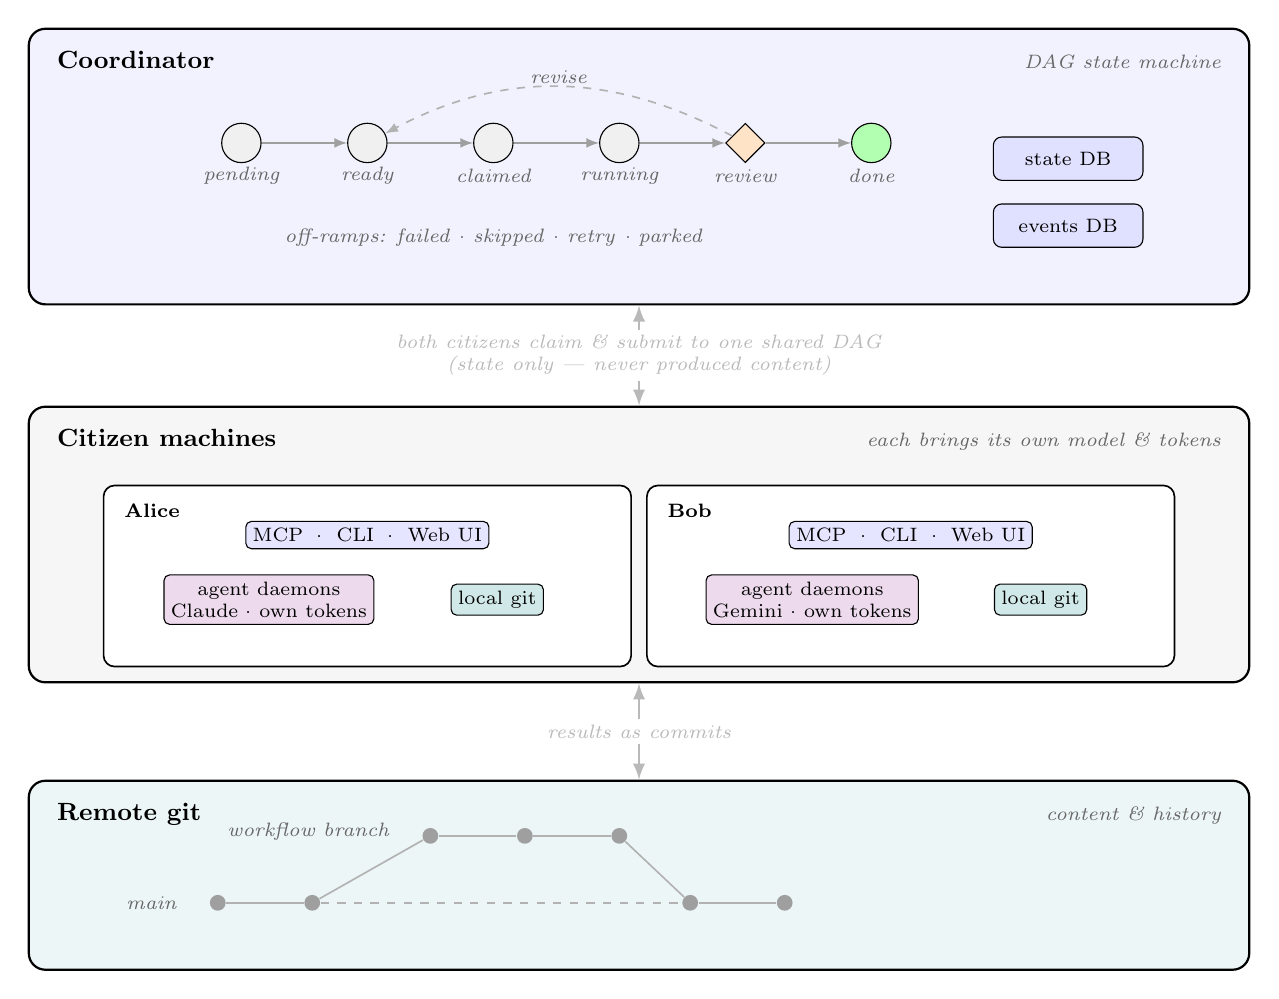
\begin{tikzpicture}[
    font=\small,
    coordband/.style={rectangle, rounded corners=6pt, draw, fill=blue!5, line width=0.8pt},
    fcband/.style={rectangle, rounded corners=6pt, draw, fill=gray!7, line width=0.8pt},
    gitband/.style={rectangle, rounded corners=6pt, draw, fill=teal!7, line width=0.8pt},
    citizen/.style={rectangle, rounded corners=4pt, draw, fill=white, line width=0.6pt},
    st/.style={circle, draw, fill=gray!12, minimum size=5mm, inner sep=0pt},
    gate/.style={diamond, draw, fill=orange!22, aspect=1.25, minimum size=5mm, inner sep=0pt},
    done/.style={circle, draw, fill=green!30, minimum size=5mm, inner sep=0pt},
    db/.style={rectangle, rounded corners=3pt, draw, fill=blue!12, minimum width=1.9cm, minimum height=0.55cm, font=\scriptsize, inner sep=2pt},
    chip/.style={rectangle, rounded corners=2pt, draw, fill=blue!10, font=\scriptsize, inner sep=2.5pt},
    daemon/.style={rectangle, rounded corners=2pt, draw, fill=violet!14, font=\scriptsize, inner sep=2.5pt, align=center},
    lgit/.style={rectangle, rounded corners=2pt, draw, fill=teal!18, font=\scriptsize, inner sep=2.5pt},
    commit/.style={circle, fill=gray!75, minimum size=2mm, inner sep=0pt},
    flow/.style={->, >=latex, gray!75, semithick},
    tie/.style={<->, >=latex, line width=1pt, gray!55},
    lbl/.style={font=\scriptsize\itshape, text=black!60},
    blab/.style={font=\bfseries\small}
]
% ----- Tier 1: Coordinator -----
\node[coordband, minimum width=15.5cm, minimum height=3.5cm] (coord) at (7.75,7.4) {};
\node[blab, anchor=north west] at ([shift={(0.25,-0.18)}]coord.north west) {Coordinator};
\node[lbl, anchor=north east] at ([shift={(-0.25,-0.22)}]coord.north east) {DAG state machine};
\node[st]   (l1) at (2.7,7.7) {};
\node[st]   (l2) at (4.3,7.7) {};
\node[st]   (l3) at (5.9,7.7) {};
\node[st]   (l4) at (7.5,7.7) {};
\node[gate] (lg) at (9.1,7.7) {};
\node[done] (l6) at (10.7,7.7) {};
\foreach \a/\b in {l1/l2,l2/l3,l3/l4,l4/lg,lg/l6} \draw[flow] (\a) -- (\b);
\draw[flow,dashed,gray!60] (lg) to[out=152,in=28] node[lbl,above,inner sep=1pt]{revise} (l2);
\node[lbl] at (2.7,7.28) {pending};
\node[lbl] at (4.3,7.28) {ready};
\node[lbl] at (5.9,7.28) {claimed};
\node[lbl] at (7.5,7.28) {running};
\node[lbl] at (9.1,7.28) {review};
\node[lbl] at (10.7,7.28) {done};
\node[lbl] at (5.9,6.5) {off-ramps: failed \textperiodcentered\ skipped \textperiodcentered\ retry \textperiodcentered\ parked};
\node[db] (sdb) at (13.2,7.5) {state DB};
\node[db] (edb) at (13.2,6.65) {events DB};
% ----- Tier 2: Citizen machines -----
\node[fcband, minimum width=15.5cm, minimum height=3.5cm] (fc) at (7.75,2.6) {};
\node[blab, anchor=north west] at ([shift={(0.25,-0.18)}]fc.north west) {Citizen machines};
\node[lbl, anchor=north east] at ([shift={(-0.25,-0.22)}]fc.north east) {each brings its own model \& tokens};
\node[citizen, minimum width=6.7cm, minimum height=2.3cm] (alice) at (4.3,2.2) {};
\node[blab, anchor=north west, font=\bfseries\scriptsize] at ([shift={(0.15,-0.12)}]alice.north west) {Alice};
\node[chip]   at (4.3,2.72) {MCP \;\textperiodcentered\; CLI \;\textperiodcentered\; Web UI};
\node[daemon] at (3.05,1.9) {agent daemons\\Claude \textperiodcentered\ own tokens};
\node[lgit]   at (5.95,1.9) {local git};
\node[citizen, minimum width=6.7cm, minimum height=2.3cm] (bob) at (11.2,2.2) {};
\node[blab, anchor=north west, font=\bfseries\scriptsize] at ([shift={(0.15,-0.12)}]bob.north west) {Bob};
\node[chip]   at (11.2,2.72) {MCP \;\textperiodcentered\; CLI \;\textperiodcentered\; Web UI};
\node[daemon] at (9.95,1.9) {agent daemons\\Gemini \textperiodcentered\ own tokens};
\node[lgit]   at (12.85,1.9) {local git};
% ----- Tier 3: Remote git -----
\node[gitband, minimum width=15.5cm, minimum height=2.4cm] (rg) at (7.75,-1.6) {};
\node[blab, anchor=north west] at ([shift={(0.25,-0.18)}]rg.north west) {Remote git};
\node[lbl, anchor=north east] at ([shift={(-0.25,-0.22)}]rg.north east) {content \& history};
\node[lbl, anchor=east] at (2.0,-1.95) {main};
\node[lbl, anchor=east] at (4.7,-1.05) {workflow branch};
\node[commit] (m1) at (2.4,-1.95) {};
\node[commit] (m2) at (3.6,-1.95) {};
\node[commit] (m3) at (8.4,-1.95) {};
\node[commit] (m4) at (9.6,-1.95) {};
\node[commit] (w1) at (5.1,-1.1) {};
\node[commit] (w2) at (6.3,-1.1) {};
\node[commit] (w3) at (7.5,-1.1) {};
\draw[gray!60,semithick] (m1)--(m2);
\draw[gray!60,semithick] (m3)--(m4);
\draw[gray!60,semithick,dashed] (m2)--(m3);
\draw[gray!60,semithick] (m2)--(w1);
\draw[gray!60,semithick] (w1)--(w2)--(w3);
\draw[gray!60,semithick] (w3)--(m3);
% ----- inter-tier ties -----
\draw[tie] (coord.south) -- (fc.north) node[midway, fill=white, inner sep=2pt, align=center, font=\itshape\scriptsize]{both citizens claim \& submit to one shared DAG\\(state only --- never produced content)};
\draw[tie] (fc.south) -- (rg.north) node[midway, fill=white, inner sep=2pt, font=\itshape\scriptsize]{results as commits};
\end{tikzpicture}
\end{document}
